\section{Overview}

\begin{frame}{\insertsection}
    \begin{table}[]
        \centering
        \renewcommand{\arraystretch}{2} % 1.5 times the default row height
        \begin{tabular}{>{\centering\bfseries}m{2cm}|>{\centering}m{4.5cm}|>{\centering\arraybackslash}m{4.5cm}|}
        \multicolumn{1}{c}{} & \multicolumn{1}{c}{\textbf{Part \RN{1}}} & \multicolumn{1}{c}{\textbf{Part \RN{2}}} \\
        \cline{2-3}
        \textbf{Phase A} & MAS ontology & gamification ontology \\
        \cline{2-3}
        \textbf{Phase B} & MAS framework & gamification framework \\
        \cline{2-3}
        \end{tabular}
        \caption{Research in a nutshell: two parts, two phases each}
        \label{tbl:research-quick-overview}
    \end{table}
\end{frame}

\begin{frame}{\insertsection}
    \customFigure[.5]{% how wide is the figure?
        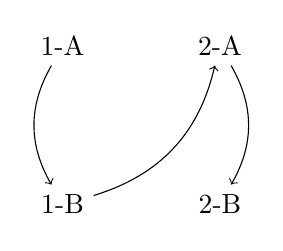
\begin{tikzpicture}
  \node (1) at (0,0) {\RN{1}-B};
  \node (2) at (2,0) {\RN{2}-B};
  \node (3) at (2,2) {\RN{2}-A};
  \node (4) at (0,2) {\RN{1}-A};
  \draw [->, bend right] (1) to (3);
  \draw [->, bend left] (3) to (2);
  \draw [->, bend right] (4) to (1);
\end{tikzpicture}

    }{The flow between the parts and the phases}{fig:research-quick-overview-flow}
\end{frame}

